% Gráfico: Comparativo Geral - Nós Restantes (Total)
\begin{figure}[htbp]
\centering
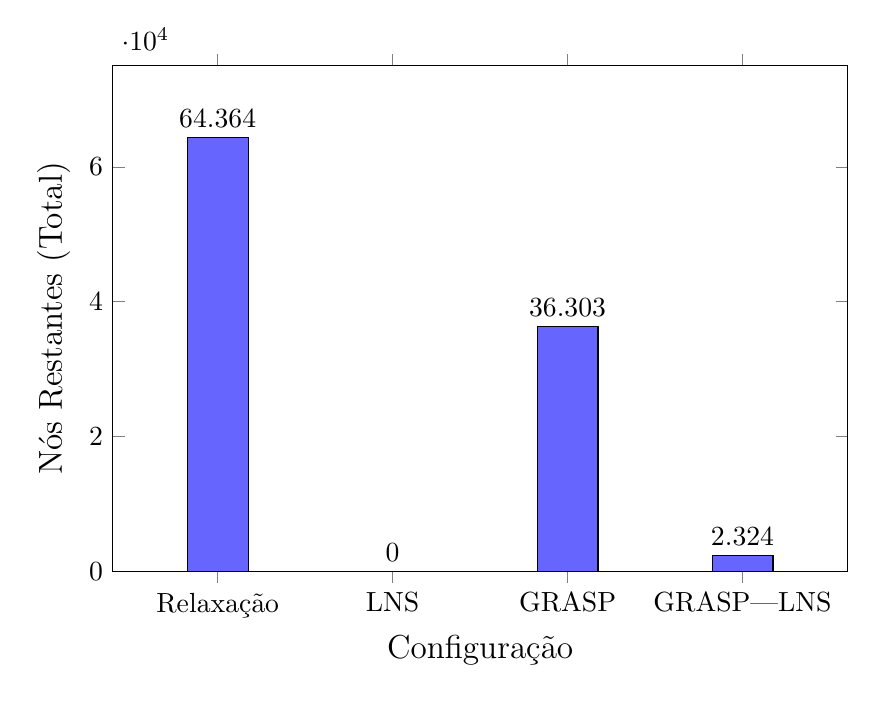
\begin{tikzpicture}
\begin{axis}[
    ybar,
    bar width=22pt,
    width=0.9\textwidth,
    height=8cm,
    ylabel={Nós Restantes (Total)},
    xlabel={Configuração},
    symbolic x coords={Relaxação, LNS, GRASP, GRASP{|}LNS},
    xtick=data,
    nodes near coords,
    nodes near coords align={vertical},
    nodes near coords style={font=\normalsize},
    every node near coord/.append style={/pgf/number format/fixed,
        /pgf/number format/precision=0,
        /pgf/number format/use comma},
    ymin=0,
    ymax=75000,
    enlarge x limits=0.2,
    ylabel style={font=\large},
    xlabel style={font=\large},
    tick label style={font=\normalsize},
]
\addplot[fill=blue!60] coordinates {
    (Relaxação,64364)
    (LNS,0)
    (GRASP,36303)
    (GRASP{|}LNS,2324)
};
\end{axis}
\end{tikzpicture}
\caption{Total de nós restantes na árvore de Branch-and-Bound para cada configuração. O LNS alcançou 0 nós restantes, resolvendo todas as instâncias até a otimalidade.}
\label{fig:geral_nodes}
\end{figure}
